\chapter{Introducción específica} % Main chapter title

\label{Chapter2}

%----------------------------------------------------------------------------------------

Este capítulo presenta en detalle los temas aplicados en el desarrollo del trabajo y las definiciones realizadas en el inicio del trabajo. Permite conocer los requisitos y organización de tareas planteados.



%----------------------------------------------------------------------------------------

\section{Requerimientos}
\label{sec:requerimientos}

A continuación,  se presentan los requerimientos planteados en la planificación del trabajo:

\begin{enumerate}
	\item Requerimientos funcionales
		\begin{enumerate}
            \item El sistema a desarrollar debe ser un prototipo funcional para pruebas en ambiente de laboratorio. 
			\item El sistema debe reportar en una plataforma de software la posición geográfica de las cavas en tiempo real.
            \item La plataforma de software deberá permitir la visualización en un mapa de la posición geográfica de las cavas.
			\item La precisión del reporte de la posición geográfica debe ser de diez metros (10 m). 
            \item Como requisito mínimo, el sistema debe ser capaz de conectarse con dos constelaciones de satélites para obtener la posición geográfica.  
            \item El hardware debe tener botones para que los operarios puedan reportar la ocupación o desocupación de las cavas. 
            \item El hardware debe poseer un display LCD que permita a los operarios visualizar las coordenadas geográficas reportadas por el sistema y el estado de ocupación de la cava. 
            \item El hardware debe poseer pilotos que permitan a los usuarios visualizar e interpretar de forma lógica el estado de ocupación de las cavas. 
		\end{enumerate}
	\item Requerimientos no funcionales
		\begin{enumerate}
			\item El sistema debe ser escalable y debe poderse replicar. 
			\item El sistema a desarrollar debe usar componentes electrónicos disponibles en Colombia. 
		\end{enumerate}
\end{enumerate}





%----------------------------------------------------------------------------------------

\section{Estructura del sistema}
\label{sec:Estructura_sistema}

En la figura ~\ref{fig:diagrama_general} se observa el diagrama general del prototipo que se construyó. Allí se representa al microcontrolador, que funge como unidad de procesamiento central. Además, se distinguen los componentes de comunicación satelital y celular: un receptor GNSS y un módulo 4G LTE. Se aprecian, las infraestructuras de comunicación que se emplearon para hacer posible la comunicación. Se distingue la infaltable fuente de alimentación para garantizar la energía. Por último, el sistema comprende de una interfaz web como herramienta para la presentación y seguimiento de la información. 

En el capítulo siguiente se aborda con más detalle la implementación de cada uno de estos módulos.


\vspace{1cm}

\begin{figure}[htbp]
	\centering
	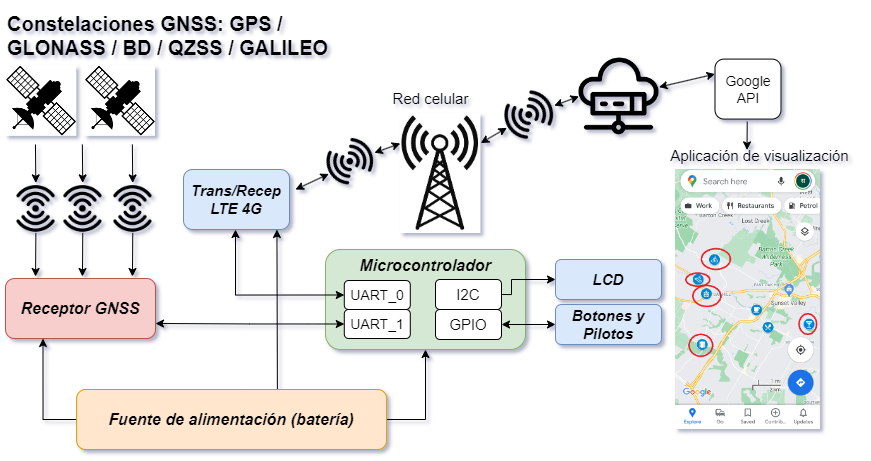
\includegraphics[width=1\textwidth]{./Figures/diagrama_general.png}
	\caption{Diagrama general del sistema.}
	\label{fig:diagrama_general}
\end{figure}


%----------------------------------------------------------------------------------------

\section{Componentes del sistema}
\label{sec:Componentes_sistema}

En este trabajo se desarrolló un prototipo para realizar el posicionamiento geográfico de cavas móviles de transporte de alimentos. Dicho sistema comprende los siguientes componentes:

\begin{itemize}
    \item Microcontrolador, que realiza las labores de unidad central de procesamiento.
    \item Receptor GNSS, para la recepción de datos de posicionamiento.
    \item Módulo de comunicación 4G, para la conexión a Internet.
    \item Plataforma de software para la presentación de la información. 
    \item Fuente de alimentación.
\end{itemize}

Para la selección de los principales componentes se buscaron alternativas en el mercado a partir de los requisitos planteados en la sección ~\ref{sec:requerimientos}.

\subsection{Microcontrolador ESP32}
\label{Microcontrolador}

Luego de realizar un estudio comparativo entre tres plataformas de microcontroladores disponibles en el mercado colombiano, se seleccionó el microcontrolador ESP32. En la tabla ~\ref{tabla:comparativa} se presenta un extracto de la comparación entre las plataformas. 

\begin{table}[h]
    \centering
    \caption{Tabla comparativa de Microcontroladores.}
    \begin{tabular}{p{3cm} p{3cm} p{2.5cm} p{2.5cm} }
    \toprule

        \textbf{Característica}           & \textbf{ESP-WRoom-32}               & \textbf{Arduino MEGA}               & \textbf{STM32 F401} \\
        \midrule
        \textbf{CPU}                    & Dual-core Tensilica Xtensa LX6     & ATmega2560 (8-bit)                  & ARM Cortex-M4 @ 84 MHz               \\
        
        \textbf{Número de núcleos}       & 2                                  & 1                                  & 1                                   \\
        
        \textbf{Frecuencia del procesador (MHz)}  & 160                       & 16                                 & 84                                  \\

        \textbf{ROM}             & 448 kB                             & 256 kB (Flash)                     & 512 kB (Flash)                      \\

        \textbf{RAM}             & 520 kB                             & 8 kB (SRAM)                        & 96 kB (SRAM)                        \\

        \textbf{Comunicación} & Wi-Fi, Bluetooth, 2x UART, 1x SPI, 1x I2C y 1x USB.    & 1x USB, 2x UART, 1x SPI e 1x I2C                 & 3x USART, 4x SPI, 3x I2C, 1x CAN y 1x USB  \\

        \textbf{Lenguajes de programación} & Arduino, C/C++ y Micropython  & Arduino y C/C++               & Arduino y C/C++                  \\

        \textbf{Cantidad de GPIO's }       & 36            & 54 (Digital), 16 (Analog)           & 82                                  \\

        \textbf{Soporte de hardware para RTOS} & Sí        & No 16 (Analog)           & Sí                                 \\
    \bottomrule
    \hline
    \end{tabular}
    \label{tabla:comparativa}
\end{table}


El microcontrolador ESP32 comprende una familia o serie de microcontroladores tipo System on Chip (SoC), desarrollado por la empresa Espressif \citep{ESPRESSIF}. 

El ESP32 es un sistema de doble núcleo con dos CPU Harvard Architecture Xtensa LX6. Toda la memoria integrada, la memoria externa y los periféricos se encuentran en el bus de datos y/o el bus de instrucciones de estas CPU. Las dos CPU se denominan PRO\_CPU y APP\_CPU (de protocolo y aplicación), sin embargo, para la mayoría de los propósitos las dos CPU son intercambiables \citep{ESPRESSIF}.

Entre las principales características de este microcontrolador se encuentran:

\begin{itemize}
    \item Espacio de direcciones de 4 GB (32 bits) para el bus de datos y el bus de instrucciones. 
    \item Espacio de direcciones DMA de 328 kB. Trece de sus módulos son capaces de operar con DMA.
    \item Espacio de direcciones periférico de 512 kB.
    \item ROM interna de 448 kB.
    \item SRAM interna de 520 kB.
    \item Admite hasta 16 MB de Flash SPI o hasta 8 MB de SPI SRAM.    
\end{itemize}

En la figura ~\ref{fig:ESP32} se presenta la placa de desarrollo ESP32-Devkit-V4.

\vspace{1cm}

\begin{figure}[htbp]
	\centering
	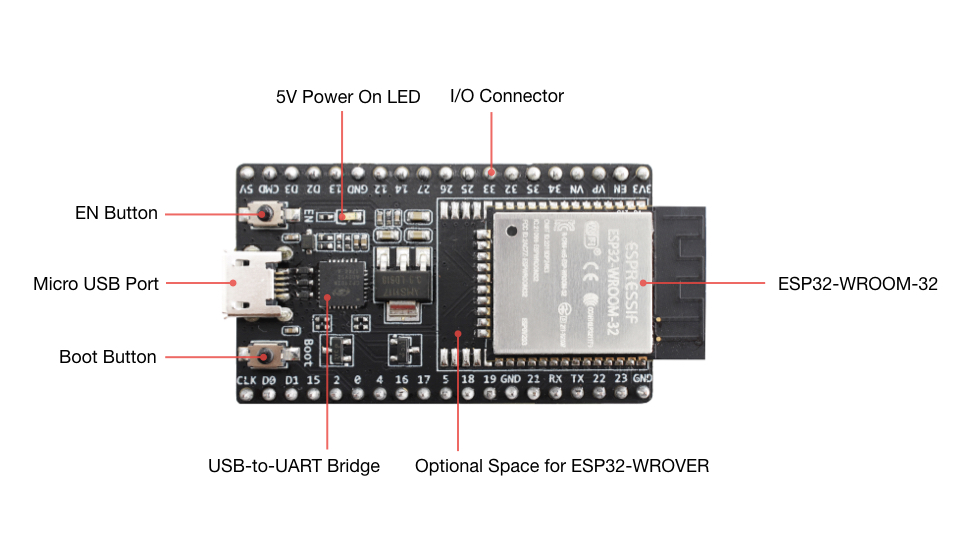
\includegraphics[width=1\textwidth]{./Figures/ESP32.jpg}
	\caption{Placa de desarrollo ESP32-Devkit-V1\protect\footnotemark.}
        
	\label{fig:ESP32}
\end{figure}
\footnotetext{Imagen tomada de: \url{https://docs.espressif.com/projects/esp-idf/en/latest/esp32/hw-reference/esp32/get-started-devkitc.html}}

A continuación, se presentan los beneficios de haber aplicado el microcontrolador ESP32 en el presente trabajo:

\begin{itemize}
    \item Es de resaltar la significativa capacidad de cómputo inherente a su diseño, ya que cuenta con un procesador de doble núcleo. Esto fue especialmente útil para implementar multitarea a través de FreeRTOS.
    \item Incorpora dos módulos de comunicación inalámbrica: Wi-Fi y Bluetooth. Esto permite la conexión con Internet y la conexión en redes de área personal. 
    \item Otro punto a favor importante para los requerimientos del trabajo, es que presenta modos de bajo de consumo energético configurables. 
    \item El fabricante proporciona una documentación extensa de su producto. Además, provee el \textit{framework} ESP-IDF que es bastante potente y está disponible gratuitamente.  
    \item Debido a que es un producto \textit{Open Source} y \textit{Open Hardware}, goza de una comunidad de desarrolladores bastante activa y una gran disponibilidad de documentación. Estas dos características posibilitan que cualquier inconveniente que se consulte tenga una alta probabilidad de ser resuelto.  
    \item Por último, es un dispositivo de bajo costo, con un precio asequible y una relación calidad/prestaciones muy buena. Esto hizo posible abaratar los costos del trabajo. 
\end{itemize}


\subsection{Receptor GNSS}
\label{sec:QL76}

Un receptor de Sistemas de Navegación Global por Satélite (GNSS, por sus siglas en inglés) es un dispositivo que permite realizar posicionamiento global. Esto lo hace a través de la recepción de señales provenientes de distintas constelaciones de satélites. Estas señales contienen información detallada sobre la posición de un objetivo a nivel mundial, lo que ofrece precisiones que abarcan desde los 10 metros hasta los 0,1 milímetros.  

Para este trabajo se seleccionó el módulo Quectel L76 (QL76), que es un receptor GNSS que admite cinco sistemas de navegación y posicionamiento global: GPS, GLONASS, Galileo, BeiDou y QZSS. En la figura ~\ref{fig:QL76} se puede observar el aspecto físico de dicho módulo \citep{QL76}. Se eligió este debido a la disponibilidad en el mercado local y a que sus características cumplen perfectamente con los requerimientos planteados. 

\vspace{1cm}

\begin{figure}[htbp]
	\centering
	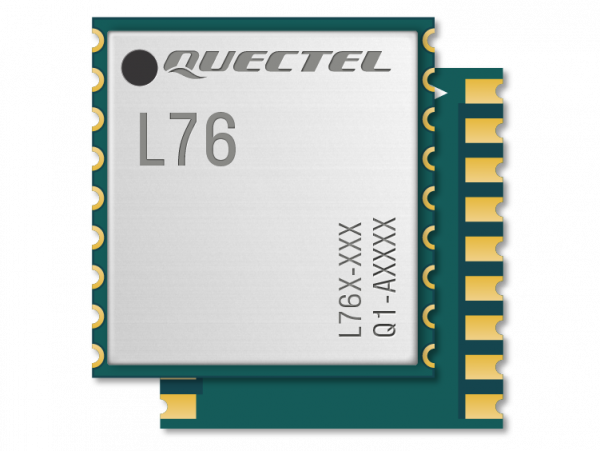
\includegraphics[width=.5\textwidth]{./Figures/QL76.png}
	\caption{Módulo Quectel L76\protect\footnotemark.}
	\label{fig:QL76}
\end{figure}
\footnotetext{Imagen tomada de: \url{https://www.quectel.com/product/gnss-l76}}

A continuación, se describen las características principales del módulo QL76 \citep{QL76}:

\begin{itemize}
    \item La configuración de constelación predeterminada es GPS+GLONASS.
    \item Admite interfaces de comunicación UART e I2C. 
    \item Ofrece diversos modos de funcionamiento que permiten la optimización del consumo de energía, a saber: GLP, AlwaysLocate™, Standby y Backup
    \item Tiene un consumo de energía extremadamente bajo.
\end{itemize}

 

\subsection{Módulo 4G}
\label{sec:SIMA7670SA}

Un transmisor/receptor 4G es un dispositivo terminal que permite la comunicación inalámbrica para dispositivos electrónicos a través de las redes de telefonía móvil de cuarta generación. Estos módulos facilitan la transmisión de datos, mensajes SMS, llamadas y conexión a internet a través de la infraestructura de redes móviles.

Para este trabajo se escogió el SoC (\textit{Sistem on Chip}) 4G SIMA7670SA con tecnología 4G. Soporta las bandas de frecuencia GSM y LTE-FDD. Está optimizado para casos de uso de IoT, diseñando bajo la especificación CAT-1. Puede oparar en condiciones difíciles, entre las que se pueden mencionar:
\begin{itemize} 
    \item Cobertura en lugares remotos.
    \item Interferencia por el fenómeno de \textit{handover}.
    \item Congestión de la red.
    \item Condiciones meteorológicas adversas. 
\end{itemize}

El SoC también integra el \textit{stack} de protocolos TCP/IP, MQTT. Este se escogió debido a que presenta buenas prestaciones en un tamaño compacto \citep{A7670SA}. 

\vspace{1cm}

\begin{figure}[htbp]
	\centering
	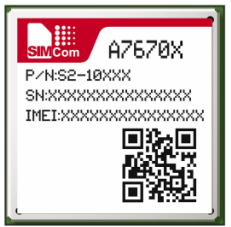
\includegraphics[width=.5\textwidth]{./Figures/A7670SA.jpg}
	\caption{Módulo SIM A7670SA\protect\footnotemark.}
	\label{fig:A7670SA}
\end{figure}
\footnotetext{Imagen tomada de: \url{https://www.simcom.com/product/A7670X.html}}

Las características principales de este SoC son: 

\begin{itemize}
    \item Frecuencias de trabajo: LTE-FDD(B1/B2/B3/B4/B5/B7/B8/B28/B66), GSM (850/900/1800/1900MHz).
    \item Soporta interfaces UART, USB, I2C y GPIO.
    \item Velocidad de descarga/carga en modo LTE de 10/5 Mbps.
    \item Velocidad de descarga/carga en modo GPRS/EDGE de 236.8/236.8 Kbps.
    \item consumo de corriente en modo LTE 3.8 mA.
    \item consumo de corriente en modo GSM 3.5 mA.
\end{itemize}

Para el presente trabajo, se utilizó el módulo A7670SA 4G LTE CAT1 MULTIBANDA GSM GPRS IOT (\textit{shield}) comercial basado en el SoC SIM A7670SA, debido a la facilidad para integrarlo al sistema general y que dispone de las interfaces de hardware necesarias para su interconexión con la ESP32, demás de su propio circuito de alimentación y un diseño fiable para evitar las interferencias electromagnéticas. Ver figura~\ref{fig:A7670SA_2}.

\begin{figure}[htbp]
	\centering
	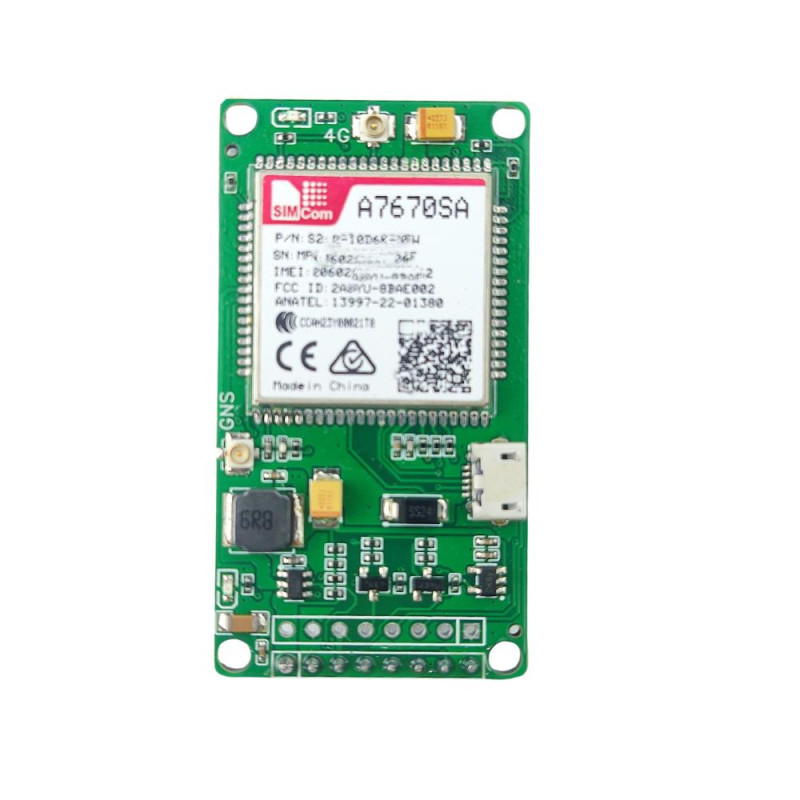
\includegraphics[width=.5\textwidth]{./Figures/A7670SA_Mod.jpg}
	\caption{Módulo A7670SA\protect\footnotemark.}
	\label{fig:A7670SA_2}
\end{figure}
\footnotetext{Imagen tomada de: \url{https://ssdielect.com/gsm-y-gprs-1/4872-a7670sa-sin-gps.html}}

\subsubsection{Antena Quectel YG0035AA}

Debido al requerimiento de conectarse, como mínimo, con dos constelaciones de satélites para obtener la posición geográfica, se debe utilizar una antena capaz de captar las frecuencias de transmisión de al menos dos constelaciones satelitales. Para este proyecto, se considera la antena Quectel YG0035AA. En la figura~\ref{fig:Antena} se observa la antena.

La antena está diseñada, según su fabricante, está diseñada con las características de alta eficiencia y excelente rendimiento. Soporta la recepción de señales de la constelación GPS y BeiDou (BD). Presenta las siguientes características eléctricas: 

\begin{itemize}
	\item Antena tipo activa.
	\item Rango de frecuencias de 1561 MHz a 1575 MHz.
	\item Impedancia de entrada de 50 ohm
	\item Ganancia entre 0.5 dBi y 1.4 dBi
	\item Polarización tipo RHCP. 
\end{itemize}

\begin{figure}[htbp]
	\centering
	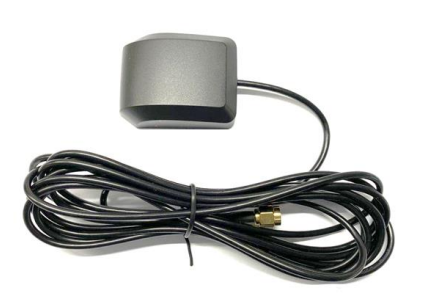
\includegraphics[width=.5\textwidth]{./Figures/Antena_Quectel_YG0035AA.png}
	\caption{Antena Quectel YG0035AA\protect\footnotemark.}
	\label{fig:Antena}
\end{figure}
\footnotetext{Imagen tomada de: \url{https://www.quectel.com/product/yg0035aa-gnss-active-magnetic-mount-antenna/}}



\subsection{Sistema operativo de tiempo real}
\label{sec:RTOS}

Un sistema operativo de tiempo real (RTOS, del inglés: Real-Time Operating System), es un tipo de sistema operativo diseñado específicamente para controlar y gestionar tareas de tiempo real en sistemas embebidos, como microcontroladores y sistemas integrados. La característica principal de un RTOS es que puede responder a eventos y ejecutar tareas de manera predecible y en un intervalo de tiempo garantizado.

El firmware que se implementó en este trabajo está basado en FreeRTOS™. En el apartado siguiente, se explica qué es y cuáles son las ventajas que se obtuvieron con su utilización. 

\subsubsection{FreeRTOS™}
\label{sec:FreeRTOS}

FreeRTOS™ es un sistema operativo de tiempo real de código abierto diseñado para sistemas embebidos y microcontroladores. Es apto para microcontroladores y microprocesadores pequeños \citep{FreeRTOS}. A continuación, se presentan las ventajas de haber implementado este sistema operativo en el trabajo.

\begin{itemize}
    \item Debido a que proporciona un kernel multitarea, permitió generar concurrencia entre tareas, como lo fueron la recepción y parseo de tramas GNSS, la transmisión de datos en tiempo real.  
    \item Gracias a la temporización precisa, se pudo asegurar la transmisión de datos de posicionamiento en tiempo real. 
    \item Permitió la gestión de la memoria y los periféricos UART del microcontrolador. De hecho, con FreeRTOS™, es posible gestionar todos los recursos del dispositivo con colas y semáforos. Al mismo tiempo, el kernel no representa una carga pesada para la capacidad de cómputo del microcontrolador utilizado. 
    \item Se pudo acceder a las ventajas de un RTOS de forma libre con la licencia MIT de FreeRTOS™.
    \item El código desarrollado es altamente portable, lo que permitirá escalar o transferir fácilmente el prototipo hacia otras plataformas. 
\end{itemize}



\subsection{Servicio web para mapas}
\label{sec:mapas_web}

Un servicio de mapas es un conjunto de herramientas y servicios de software que permiten que los mapas estén disponibles en la web. A menudo este es ofrecido por un proveedor especializado. 

Para este trabajo se creó una aplicación web basada en los servicios de Google Maps Platform \citep{GoogleMaps}. Esta utiliza la ubicación obtenida del módulo GNSS para visualizar información geográfica en un mapa de Google. 